\documentclass[aspectratio=169,10pt]{beamer}

\usepackage[UTF8]{ctex}
\usepackage{hyperref}
\usepackage{amsmath}
\usepackage{array}
\usepackage{booktabs}
\usepackage{tabularx}
\usepackage{graphicx}
\usepackage{assets/tju-course-report}

\hypersetup{
  colorlinks=true,
  urlcolor=dutBlueDark,
  linkcolor=dutBlueDark
}

\setlength{\tabcolsep}{3.5pt}
\renewcommand{\arraystretch}{1.22}

\newcommand{\smallnote}[1]{{\fontsize{7.5}{9.5}\selectfont\color{dutMuted}#1}}
\newcommand{\code}[1]{{\texttt{\small #1}}}
\newcommand{\pill}[1]{\colorbox{dutSky}{\textcolor{dutBlueDark}{\texttt{#1}}}}

\begin{document}

% 0:20 — 封面
\duttitlepage{
  基于 xv6-RISC-V 的\\
  静态优先级调度与\\
  Aging 防饥饿机制
}{操作系统设计综合实践课程汇报}{第 35 组}{2026 年 9 月}

% 0:55 — 项目目标与团队分工
\begin{dutframe}{项目概览}{先明确问题，再分工实现}
  \begin{columns}[T,totalwidth=\textwidth]
    \column{0.43\textwidth}
      \begin{dutsection}{问题与目标}
        xv6 原有轮转调度把可运行进程近似等价对待，难以表达任务之间的紧急程度。
        \vspace{0.04cm}
        \begin{itemize}
          \setlength{\itemsep}{0.10cm}
          \item 用静态优先级表达调度倾向；
          \item 保留同优先级进程的基本公平；
          \item 用 Aging 降低低优先级进程长期等待的风险。
        \end{itemize}
      \end{dutsection}
      \vspace{0.14cm}
      \begin{dutsection}{统一约定}
        \centering
        \pill{0 最高}\quad\pill{10 默认}\quad\pill{31 最低}
      \end{dutsection}
    \column{0.54\textwidth}
      \begin{dutsection}{五人分工}
        \small
        \begin{tabularx}{\linewidth}{>{\bfseries\color{dutBlueDark}}p{1.28cm} X}
          赖弈铭 & Aging、等待时间累计与防饥饿逻辑 \\
          刘文睿 & 静态优先级调度与同级公平 \\
          吴雨桐 & 测试设计、集成与回归验证 \\
          党正清 & 优先级系统调用与用户态 \code{nice} \\
          袁晟棋 & 进程字段、默认值、fork 继承与集成 \\
        \end{tabularx}
      \end{dutsection}
      \vspace{0.16cm}
      \smallnote{实现边界：保持 xv6 原有状态转换与锁语义，不引入 MLFQ、CFS 或复杂队列。}
  \end{columns}
\end{dutframe}

% 1:05 — 总体架构与优先级约定
\begin{dutframe}{总体设计}{从用户命令到调度器}
  \centering
  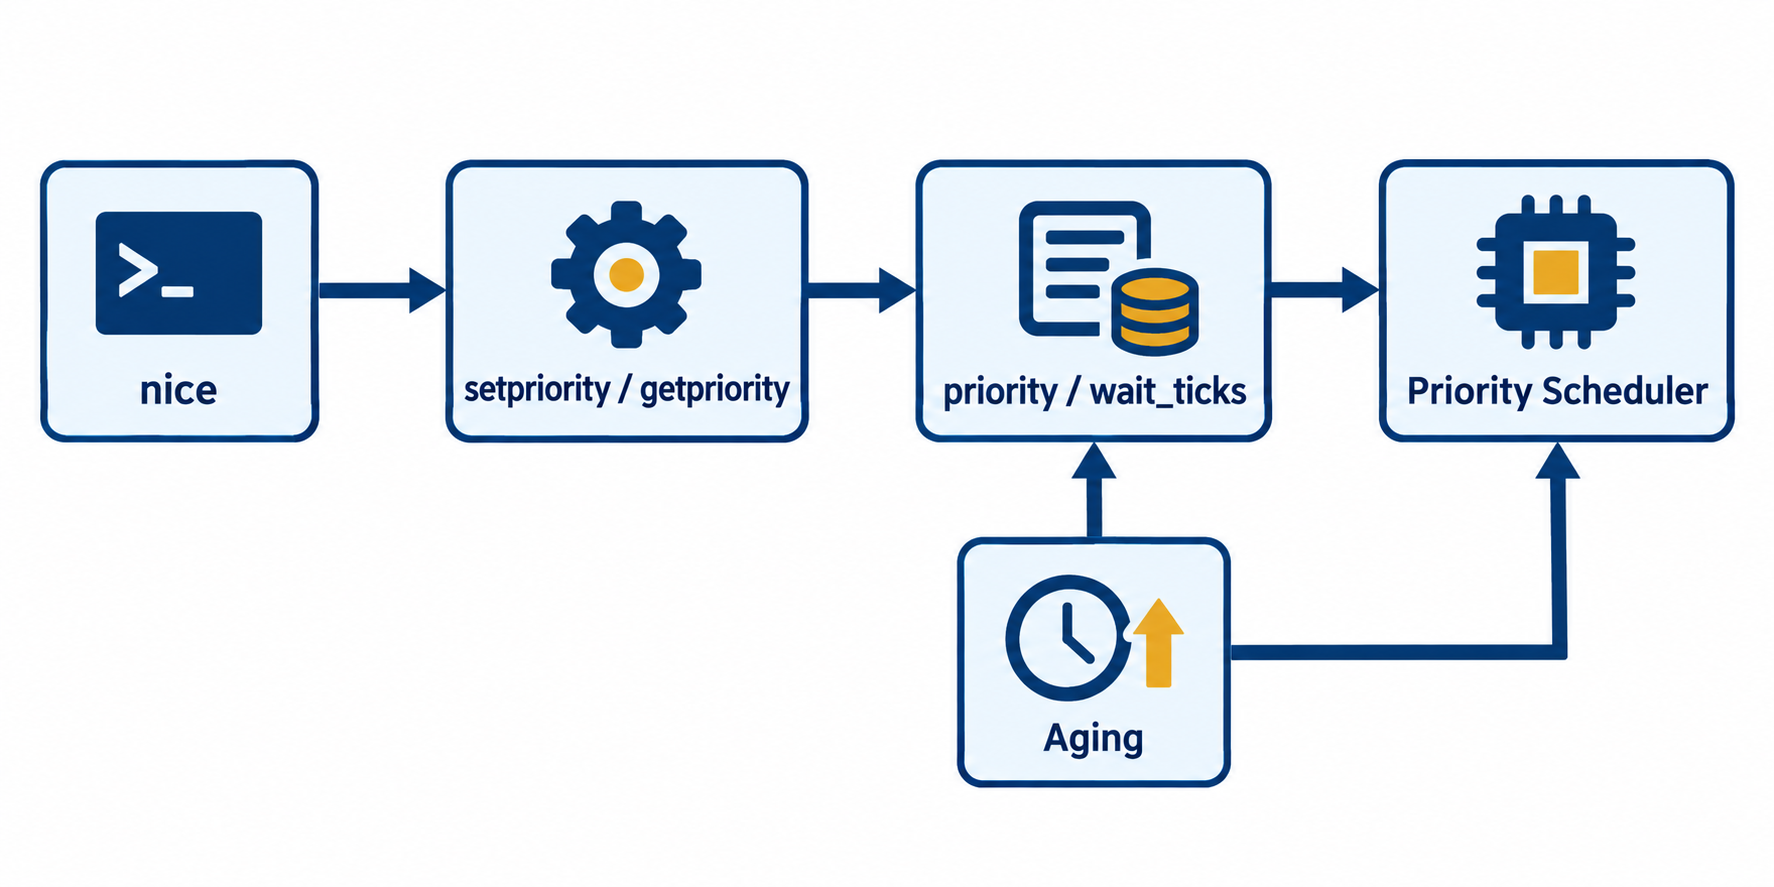
\includegraphics[width=0.62\textwidth,trim=0 0.70cm 0 1.15cm,clip]{assets/priority-architecture.png}
  \vspace{-0.22cm}
  \dutcaption{图 1  优先级控制路径：用户态命令进入系统调用，最终影响进程字段与调度选择。}
  \vspace{0.10cm}
  \begin{columns}[T,totalwidth=\textwidth]
    \column{0.31\textwidth}
      \begin{dutsection}{优先级语义}
        数字越小，优先级越高；合法范围为 $0$--$31$，默认值为 $10$。
      \end{dutsection}
    \column{0.31\textwidth}
      \begin{dutsection}{关键状态}
        \code{priority} 描述当前静态优先级，\code{wait\_ticks} 为 Aging 提供等待依据。
      \end{dutsection}
    \column{0.31\textwidth}
      \begin{dutsection}{调度入口}
        scheduler 只选择 \code{RUNNABLE} 进程，并在真正切换前再次确认状态。
      \end{dutsection}
  \end{columns}
\end{dutframe}

% 1:00 — 模块 A：进程优先级数据结构
\begin{dutframe}{}{进程优先级数据结构}
  \begin{columns}[T,totalwidth=\textwidth]
    \column{0.39\textwidth}
      \begin{dutsection}{字段设计}
        \begin{tabularx}{\linewidth}{>{\bfseries\color{dutBlueDark}}p{2.2cm} X}
          \code{priority} & 静态优先级，合法范围 $0$--$31$。 \\
          \code{wait\_ticks} & 进程处于 \code{RUNNABLE} 状态时的等待累计。
        \end{tabularx}
      \end{dutsection}
      \vspace{0.28cm}
      \begin{dutsection}{统一语义}
        \centering
        \pill{0 最高}\quad\pill{10 默认}\quad\pill{31 最低}
      \end{dutsection}
    \column{0.56\textwidth}
      \begin{dutsection}{生命周期处理}
        \small
        \begin{tabularx}{\linewidth}{>{\bfseries\color{dutBlueDark}}p{2.15cm} X}
          创建进程 & 设置默认优先级，清零 \code{wait\_ticks}。 \\
          fork 子进程 & 继承父进程优先级，等待计数重新置零。 \\
          调度成功 & 被选中的进程清零等待计数。 \\
          释放并复用 & 重置字段，避免旧状态影响新进程。
        \end{tabularx}
      \end{dutsection}
      \vspace{0.22cm}
      \begin{dutsection}{锁保护}
        \small
        fork 读取父进程优先级前先取得父进程锁，复制受保护的优先级快照。
      \end{dutsection}
  \end{columns}
\end{dutframe}

% 1:30 — 模块 B：静态优先级调度
\begin{dutframe}{}{静态优先级调度}
  \begin{dutsection}{两轮扫描}
    \small
    \begin{tabularx}{\textwidth}{>{\bfseries\color{dutBlueDark}}p{1.65cm} >{\raggedright\arraybackslash}p{5.15cm} X}
      第 1 轮 & 扫描进程表；对等待进程执行 Aging，并找出最小合法优先级。 & 先确定需要服务的优先级层。 \\
      第 2 轮 & 从 \code{next\_index} 开始循环，选择该优先级下的第一个 \code{RUNNABLE} 进程。 & 再决定这一轮由谁运行。 \\
      切换前 & 重新检查状态并获得进程锁，切换后推进 \code{next\_index}。 & 适配多 CPU，减少状态竞争和同级偏爱。
    \end{tabularx}
  \end{dutsection}
  \vspace{0.28cm}
  \begin{columns}[T,totalwidth=\textwidth]
    \column{0.47\textwidth}
      \begin{dutsection}{核心判断}
        \[
          p_{\mathrm{best}}=\min\{p.\mathrm{priority}\mid p.\mathrm{state}=\mathrm{RUNNABLE}\}
        \]
        数值越小，进程越早获得调度机会。
      \end{dutsection}
    \column{0.47\textwidth}
      \begin{dutsection}{公平性与 Aging}
        \small
        \code{next\_index} 只在同优先级候选者之间轮转；等待达到 \code{AGING\_INTERVAL=50} 后，优先级向 $0$ 方向提升一级。
      \end{dutsection}
  \end{columns}
\end{dutframe}

% 1:15 — 模块 C：系统调用与用户态命令
\begin{dutframe}{}{系统调用与用户态命令}
  \begin{columns}[T,totalwidth=\textwidth]
    \column{0.47\textwidth}
      \begin{dutsection}{接口链路}
        \small
        \begin{tabularx}{\linewidth}{>{\bfseries\color{dutBlueDark}}p{3.15cm} X}
          \code{setpriority} & 设置目标 PID 的优先级。 \\
          \code{getpriority} & 查询目标 PID 的优先级。 \\
          系统调用号 & 23 与 24，沿用 xv6 的注册流程。 \\
          用户态入口 & 在 \code{user.h}、\code{usys.pl} 中保持一致。
        \end{tabularx}
      \end{dutsection}
      \vspace{0.24cm}
      \begin{dutsection}{内核实现}
        \small
        \code{sysproc.c} 负责取参数，\code{proc.c} 在遍历进程表时逐项加锁，成功后释放锁再返回。
      \end{dutsection}
    \column{0.47\textwidth}
      \begin{dutsection}{参数检查}
        \begin{itemize}
          \setlength{\itemsep}{0.14cm}
          \item PID 必须是正数，且目标进程存在；
          \item 优先级必须满足 $0\le p\le31$；
          \item 手动设置后清零 \code{wait\_ticks}，避免旧等待历史立即触发 Aging。
        \end{itemize}
      \end{dutsection}
      \vspace{0.22cm}
      \begin{dutsection}{命令形式}
        \small
        \code{nice pid} 查询优先级；\quad\code{nice pid p} 设置优先级并打印结果。
      \end{dutsection}
  \end{columns}
\end{dutframe}

% 1:15 — 模块 D：调度统计
\begin{dutframe}{}{调度统计}
  \begin{dutsection}{测试输出的指标}
    \small
    \begin{tabularx}{\textwidth}{>{\bfseries\color{dutBlueDark}}p{2.45cm} >{\raggedright\arraybackslash}p{4.55cm} X}
      \code{METRIC} & \code{prioritytest} 输出 case、PID、优先级、起止 tick 与 work。 & 比较同级公平和不同优先级的完成先后。 \\
      \code{AGING\_RESULT} & 输出提升耗时、目标优先级、存活竞争者和超时标志。 & 直接判断 Aging 是否生效。 \\
      \code{wait\_ticks} & 仍是内核中的等待累计字段，不新增持久化调度次数。 & 保持实现边界清晰，统计由测试侧汇总。
    \end{tabularx}
  \end{dutsection}
  \vspace{0.30cm}
  \begin{columns}[T,totalwidth=\textwidth]
    \column{0.47\textwidth}
      \begin{dutsection}{当前实现边界}
        \small
        内核保留 \code{priority} 与 \code{wait\_ticks} 两个核心字段；调度次数和运行时间不写入 \code{struct proc}，避免扩大课题范围。
      \end{dutsection}
    \column{0.47\textwidth}
      \begin{dutsection}{实际回归}
        \small
        单 CPU 输出 6 条 \code{METRIC}，3 CPU 输出 12 条；两组 \code{agingtest} 和 \code{usertests -q} 均通过。
      \end{dutsection}
  \end{columns}
  \vfill
  \centering
  \small
  项目仓库：\href{https://github.com/Aphrodite-deepblue/os-design-practice}{\colorbox{dutSky}{\textcolor{dutBlueDark}{github.com/Aphrodite-deepblue/os-design-practice}}}
\end{dutframe}

% 0:30 — 模块 E：用户态测试
\begin{dutframe}{}{用户态测试}
  \begin{columns}[T,totalwidth=\textwidth]
    \column{0.53\textwidth}
      \begin{dutsection}{测试矩阵}
        \small
        \begin{tabularx}{\linewidth}{>{\bfseries\color{dutBlueDark}}p{2.35cm} >{\raggedright\arraybackslash}X}
          \code{prioritytest} & API 边界、\code{nice}、fork 继承、同级与混合优先级。 \\
          \code{agingtest} & 8 个高优先级竞争者存在时，低优先级进程逐级提升。 \\
          \code{usertests -q} & 进程退出后继续运行，检查原有 xv6 行为稳定性。
        \end{tabularx}
      \end{dutsection}
    \column{0.40\textwidth}
      \begin{dutsection}{程序与日志}
        \small
        \code{tests/run\_scheduler\_tests.py} 构建镜像、启动 QEMU，并保存原始日志、\code{results.json} 与 \code{metrics.csv}。
      \end{dutsection}
      \vspace{0.25cm}
      \begin{dutsection}{当前状态}
        \small
        单 CPU 与 3 CPU 均为 PASS；Aging 分别在 136 与 45 ticks 内完成，且未发生超时。
      \end{dutsection}
  \end{columns}
  \vfill
  \centering
  \smallnote{结果来自当前 main 快照的真实 QEMU 回归；不将一次运行当作性能基准。}
\end{dutframe}

% 0:10 — 独立结尾页
\dutclosingpage{谢谢大家}{第 35 组\quad · \quad 天津大学软件学院}

\end{document}
